%%%%%%%%%%%%%%%%%%%%%%%%%%% asme2ej.tex %%%%%%%%%%%%%%%%%%%%%%%%%%%%%%%
% Template for producing ASME-format journal articles using LaTeX    %
% Written by   Harry H. Cheng, Professor and Director                %
%              Integration Engineering Laboratory                    %
%              Department of Mechanical and Aeronautical Engineering %
%              University of California                              %
%              Davis, CA 95616                                       %
%              Tel: (530) 752-5020 (office)                          %
%                   (530) 752-1028 (lab)                             %
%              Fax: (530) 752-4158                                   %
%              Email: hhcheng@ucdavis.edu                            %
%              WWW:   http://iel.ucdavis.edu/people/cheng.html       %
%              May 7, 1994                                           %
% Modified: February 16, 2001 by Harry H. Cheng                      %
% Modified: January  01, 2003 by Geoffrey R. Shiflett                %
% Use at your own risk, send complaints to /dev/null                 %
%%%%%%%%%%%%%%%%%%%%%%%%%%%%%%%%%%%%%%%%%%%%%%%%%%%%%%%%%%%%%%%%%%%%%%

%%% use twocolumn and 10pt options with the asme2ej format
\documentclass[twocolumn,10pt]{asme2ej}

\usepackage{epsfig} %% for loading postscript figures
\usepackage[font=small,labelfont=bf]{caption}
\usepackage{enumitem}
\usepackage{amsmath} % for "bmatrix" environment and "\dfrac" macro
\usepackage{relsize}
\usepackage{float}
\usepackage{courier}
\usepackage{xcolor}

\setlength{\parindent}{0pt}
\newcommand{\id}{\hspace{6 mm}}
%\newcommand{\hypotenuse}{$a^{2}+b^{2}$}


\raggedbottom

\title{Low-Cost Visible Light Spectral Imaging}


\author{Daniel W. Dichter
    \affiliation{
Independent Researcher\\
Cambridge, Massachusetts, U.S.A.\\
daniel.w.dichter@gmail.com
    }	
}

\begin{document}

\maketitle

\color{red}
\emph{\textbf{DRAFT: \today}}\\
\color{black}

\begin{abstract}{\it Spectral imaging is an emerging technology for measuring spectral power distributions (SPDs) of electromagnetic radiation over a 2D spatial domain. Within the visible light wavelength band, spectral imaging measures light and color with greater accuracy than conventional cameras. However, adoption of this technology is impeded by high cost and complexity. To address these barriers, a simple low-cost method is developed using unmodified commodity hardware --- primarily a DSLR camera and a series of narrow bandpass filters. The quantity of filters is strictly minimized to a total of seven, set by the dimensionality of SPDs, the spectral sensitivities of eyes and cameras, and commercial availability. Camera spectral sensitivity is measured using this same filter series, a color chart, a spectrophotometer, and noon daylight modeled as CIE D65. The RAW photo format is used to access unprocessed 14-bit sensor data. Independent SPD measurements from each color channel are fused as a sensitivity-weighted average for efficient and continuous interpolation between color channels with a bias toward maximal signal-to-noise ratio. Images are reconstructed from SPDs with standard methods. The method is demonstrated with a Canon 650D camera, ThorLabs 1'' narrow bandpass filters, an X-Rite ColorChecker chart, and a Spectro 1 spectrophotometer. Accuracy is verified by quantitative comparison against SPDs from direct measurement, and by qualitative assessment of reconstructed images. The total hardware cost is \$1,500 from scratch, or \$800 starting with a camera of known spectral sensitivity.
}
\end{abstract}

\section{Introduction}

\subsection{Background}

% Motivate spectral imaging generally

Color perception results from the interaction of an illuminant, optionally a reflective surface, and an observer. Humans are \textit{trichromats}, having three-dimensional color perception, over the visible light wavelength spectrum of 400 to 700 nm. Various animal species are \textit{dichromats}, \textit{tetrachromats}, and so on, with differing visible light wavelength limits. As discussed in Section \ref{curve_reconstruction}, human color perception is significantly rank-deficient even within its limited wavelength limits.

% Overview of hyperspectral datacubes

\id Whereas conventional digital photography produces a three-dimensional RGB color image, spectral imaging produces an N-dimensional \textit{hyperspectral datacube} (HSDC), typically with 10 $\leq$ N $\leq$ 60; wavelength channels replace color channels. Because HSDCs are informationally complete and observer independent, they provide a more accurate representation of color, and enable greater optionality in subsequent image processing.

% Spectral scanning

\id \textit{Spectral scanning} is the simplest of several methods of generating HSDCs, wherein a 1-channel intensity image is captured at a series of regularly-spaced, narrow, non-overlapping wavelength bands; these images are subsequently ``stacked'' to form the final HSDC. Though spatially high-resolution relative to other methods, spectral scanning experiences ``spectral smearing'' if the subjects or sensor move during the image capture process, due to the characteristically large temporal distribution of the images. By comparison, various so-called ``single-shot'' methods use filtering techniques to capture the entire HSDC simultaneously, but at lower spatial resolution.

% Cameras

\id Commercially-available hyperspectral cameras typically cost in excess of \$15,000, whereas commodity consumer cameras such as DSLRs cost approximately \$500-1,500. DSLRs are not capable of spectral imaging as-is, but various investigators have demonstrated this capability nonetheless with various hardware and software methods. All such methods account for the non-linear trichromate spectral sensitivity of the camera's Bayer filter and image sensor.

\subsection{Related Work}

 Several authors have demonstrated spectral imaging with ordinary cameras.

\id Cosentino \cite{Cosentino} used 12 bandpass filters and a consumer camera to produce HSDCs, comparing results favorably to a commercial spectral imaging system. The method requires modification of the camera, the filters are of non-uniform properties, and the quantity of filters is larger than necessary.

\id Baek et al. \cite{Baek} developed a single-shot method using a custom prism objective to induce diffraction grating. Computation then separates the combined spatial and wavelength information by detection of ``spectral cues'' present ``only around object edges''. The requirement for the presence of edges limits the scenes that may be captured, and leads to a sensitive dependence between scene and system accuracy.

\id Habel et al. \cite{Habel} similarly developed a single-shot diffraction grating method. The custom objective is rather large and complex, and the reconstructed images are limited to 120 x 120 pixels.

\id Oh et al. \cite{Oh} developed a method using three different digital cameras, exploiting small variations in camera sensitivities. An image registration process is used to align images between cameras using planarity. PCA is performed on a spectral database of Munsell colors to create a vector space for describing SPDs as low-dimension linear combinations.

\section{Methods}

\subsection{Dimensionality of Reflectance Spectra}

Parkkinen et al. \cite{Parkkinen} measured the reflectance spectra of 1,257 standard Munsell color chips over 400 to 700 nm. Noting that ``the components of a color spectrum are highly correlated'', Parkkinen et al. performed principal component analysis on these spectra, producing a set of reflectance eigenvectors. It was found that these reflectances could be reconstructed accurately as linear combinations of no more than eight eigenvectors, though the exact quantity depends on the required accuracy. This result implies that reflectance spectra are approximately eight-dimensional over the visible light spectrum, with a characteristic wavelength resolution of approximately (700 nm - 400 nm) / 8 = 37.5 nm.

\subsection{Curve Reconstruction}
\label{curve_reconstruction}

Sampling an SPD by spectral scanning with narrow bandpass filters produces a ``sparse'' sample; the value of the SPD is measured only at certain regular intervals. In the intervals between measurements, the value of the SPD is not measured, but can be accurately inferred due to the limited dimensionality of SPDs. This process is modeled as a curve reconstruction problem, i.e. given a sparse sampling of an unknown curve, reconstruct the curve by means of an appropriate interpolation scheme such that the reconstructed curve matches a theoretical measured curve.

\id To determine the optimal filter quantity and interpolation scheme, two reflectance datasets are considered: the 8 eigenvectors developed by Parkkinen \cite{Parkkinen}, and the 24 spectra measured from an X-Rite ColorChecker Classic (2014) using a Spectro 1 spectrophotometer. The quality of the reconstruction is calculated as the residual sum of squares, multiplied by the wavelength resolution, divided by the quantity of samples in the dataset. This calculation is performed without an illuminant (i.e. directly on reflectance), and with CIE D65 representing typical noon daylight. This normalized error metric allows direct comparison between datasets. It is assumed that the filters are of sufficiently narrow bandwidth that they permit curve measurement exactly at their center wavelength.

\id Table \ref{table_reconstruction} organizes these results into four subsets with a common illuminant and reflectance. The follow observations are made:

\begin{enumerate}
  \item 30 nm resolution outperforms 40 nm resolution in all cases.
  \item With a 40 nm resolution, cubic interpolation is optimal.
  \item With a 30 nm resolution, cubic interpolation is at least near-optimal.
  \item Optimized error at 40 nm is 1-3x the optimized error at 30 nm, but both are small in an absolute sense.
  \item The inclusion (or exclusion) of an illuminant does not significantly affect the quality of the curve reconstruction; reflectance dominates.
\end{enumerate}

Thus, 40 nm resolution and cubic interpolation are used for curve reconstruction. Representative plots are shown in Figure \ref{colorchecker_reconstruction}.

\subsection{Filter Set Selection}

\label{section_filters}

Manufacturers of narrow bandpass filters include ThorLabs, Edmund Optics, and MidOpt. Within the visible light spectrum, filter center wavelength (CWL) is generally discretized as whole-number multiples of 10 nm, i.e. [400, 410, 420, ... 700] nm.

\id The centroid of the visible light spectrum may be defined at the wavelength corresponding to 50\% on the cumulative density function (CDF) of the CIE 2° tristimulus observer functions $\mathrm{\bar{x}}$, $\mathrm{\bar{y}}$, and $\mathrm{\bar{z}}$. Rounding to the nearest 10 nm per commercial availability, this centroid is 540 nm.

\id It can be shown that the wavelength range of 420 to 660 nm encompasses 97\% of the area under the CIE 2° and 10° observer functions. This range is also evenly divisible into 40 nm increments, and intersects the centroid of 540 nm.

\id The final specification is the full-width half max (FWHM), or bandwidth. As discussed in Section \ref{curve_reconstruction}, it is desirable to minimize FWHM so that measurements are wavelength-accurate. The associated reduction in overall transmission can be compensated for by increasing the brightness of the exposure, as discussed in Section \ref{photographic}.

\id The set of filters chosen are shown in Figure \ref{thorlabs_filter_transmission_spectra}, and have the following properties:\\

\begin{tabular}{l | l}
%\hline
Quantity & 7 \\
Manufacturer & ThorLabs \\
CWL & 420 to 660 nm in 40 nm increments \\
FWHM & 10 nm each \\
Part Numbers & FB420-10, FB460-10, etc. \\
Diameter & 1'' \\
Cost, Total & \$700 \\
%\hline
\end{tabular}

\begin{figure}
\centering
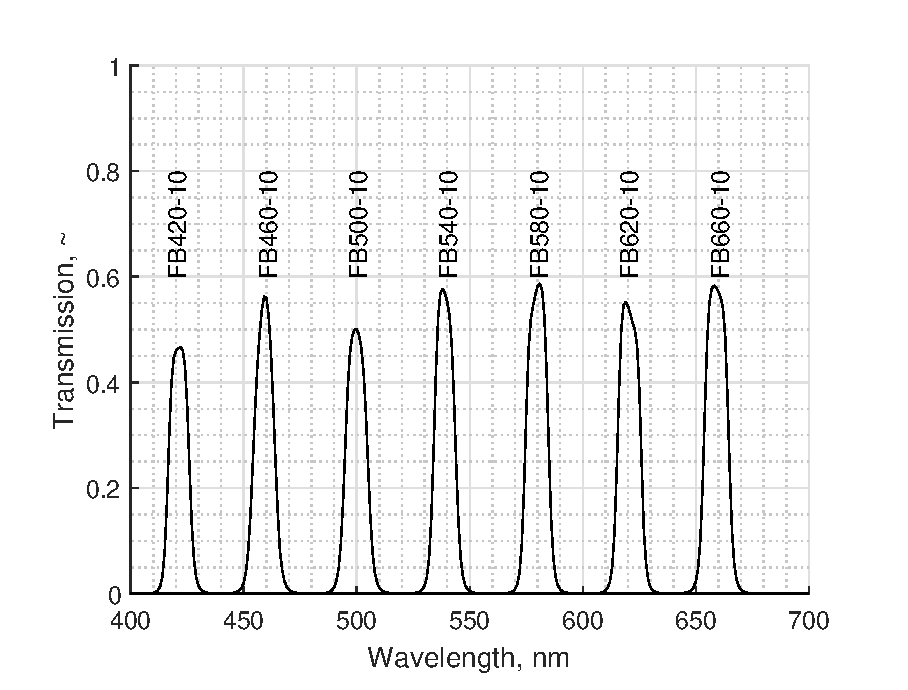
\includegraphics[width=0.5\textwidth]{thorlabs_filter_transmission_spectra.eps}
\caption{ThorLabs narrow bandpass filter transmission spectra.}
\label{thorlabs_filter_transmission_spectra}
\end{figure}

\subsection{Camera Spectral Sensitivity}

\label{Camera_Spectral_Sensitivity}

Camera spectral sensitivity is calculated by photographing a color chart of known reflectance through each filter under cloudless noon daylight modeled as CIE D65. Each color swatch produces a unique SPD modeled as the element-wise product of its spectral reflectance with the CIE D65 illuminant. An X-Rite ColorChecker was used, containing 24 swatches that mimic everyday spectral reflectances. The spectral reflectances were measured using a Spectro 1 spectrophotometer.

\id Assuming a linear response between quantity of photons incident on the sensor during an exposure, and the measured RAW value, sensitivity may be described generally as:\\

$\mathrm{ Sensitivity = S = \dfrac{Value \ Measured}{Value \ Actual} } = \dfrac{V_M}{V_A}$ \\

$V_A = \mathlarger{\sum_{\lambda}} I(\lambda) R(\lambda) T(\lambda)$ \\

 with: \\

\begin{tabular}{l | l}
$\lambda$ & Wavelength \\
I & Illuminant\\
R & Reflectance \\
T & Transmission \\
\end{tabular} \\

$V_M$ is calculated as the mode of the values inside a square inset slightly from the swatch borders.

\id Theoretically, sensitivity for all color channels and wavelengths can be calculated from any single swatch, as shown in Figure \ref{canon_650d_sensitivity}. These per-swatch sensitivity curves are fused as a weighted average using $V_M$. This has the effect of weighting calculated sensitivities in proportion to their signal-to-noise ratio (SNR).

\id The final result is a set of three sensitivity curves, $S_R(\lambda), \ S_G(\lambda), \ S_B(\lambda)$. As shown in Figure \ref{camera_spectral_sensitivities}, this result is consistent with values from literature for similar Canon cameras. \cite{Jiang}

\begin{figure}
\centering
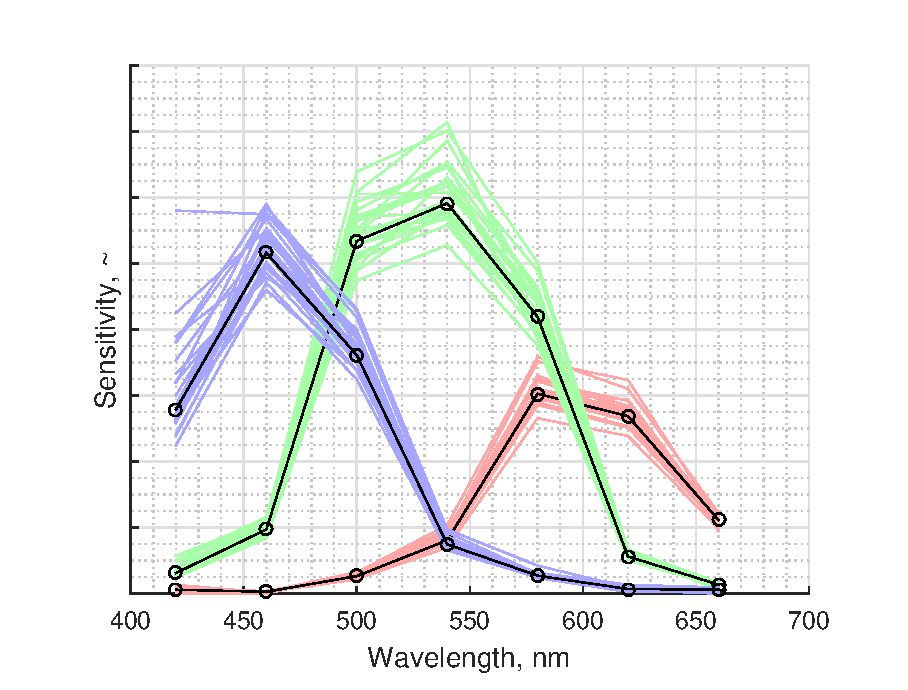
\includegraphics[width=0.5\textwidth]{canon_650d_sensitivity.eps}
\caption{Trichromate spectral sensitivity of Canon 650D camera from ColorChecker under D65 illuminant. Faint colored lines correspond to individual swatches; solid black lines correspond to per-wavelength averages for all swatches.}
\label{canon_650d_sensitivity}
\end{figure}

\begin{figure}
\centering
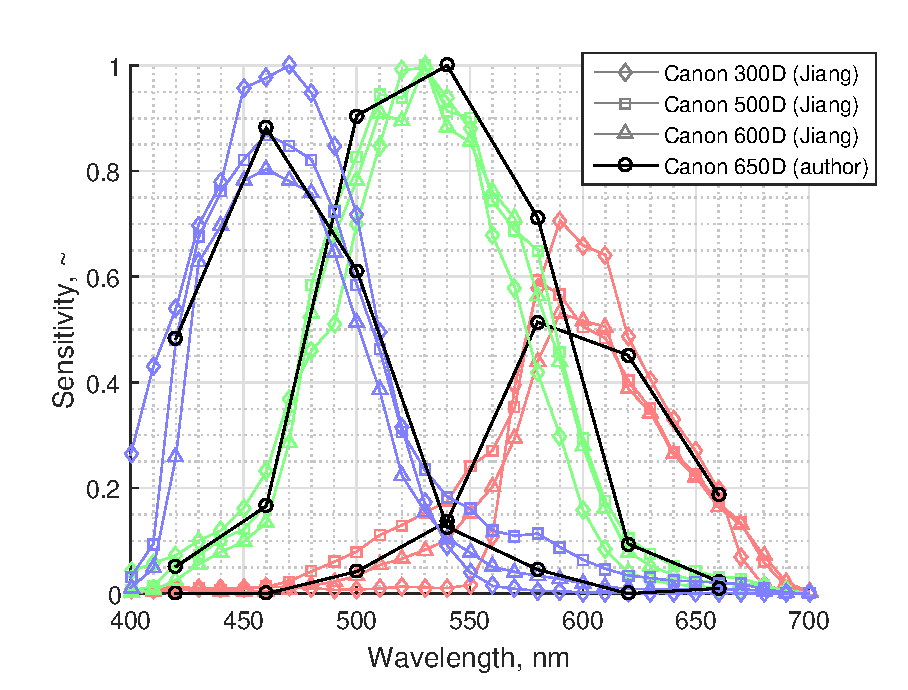
\includegraphics[width=0.5\textwidth]{camera_spectral_sensitivities.eps}
\caption{Comparison of normalized sensitivities for various Canon cameras between this paper and literature. \cite{Jiang}}
\label{camera_spectral_sensitivities}
\end{figure}

\subsection{Photographic Aspects}
\label{photographic}

 A prime lens, tripod, and remote shutter are used to minimize movement of the camera while capturing the photo stack. Because filter cost is proportional to filter area, the choice of lens is thus a significant means of cost reduction. The measurement of interest is the diameter of the objective at the outer end of the lens. For consumer-grade Canon EF lenses, this ranges from approximately 20 to 60 mm. The theoretical filter cost at these extremes differs by nearly an order of magnitude; $60^2 / 20^2 = 9$.

\id The lens selected has an outer objective diameter of 20 mm, a focal length of 40 mm, and an aperture of f/2.8. It is shown in Figure \ref{canon_40_mm_prime_lens}.

\id The filters discussed in Section \ref{section_filters} are unthreaded, and used by resting them against the camera lens by hand. The lens is designed such that the glass optics are recessed slightly from the exterior body against which the lenses rest. The filters are stored in a case in order of ascending wavelength, and cycled through in sequence to capture the photo stack.

\id The fastest aperture of f/2.8 is used. Depending on the amont of light within the scene, the ISO ranges from 100-400, and the shutter speed ranges from 1/4 to 1/500 of a second. These bright exposures are required to compensate for the low transmission of the filters. The settings are collectively adjusted to ``expose to the right'', i.e. fully utilize the available set of values without saturating the upper limit, thereby maximizing the signal-to-noise ratio in the measured values.

\begin{figure}
\centering
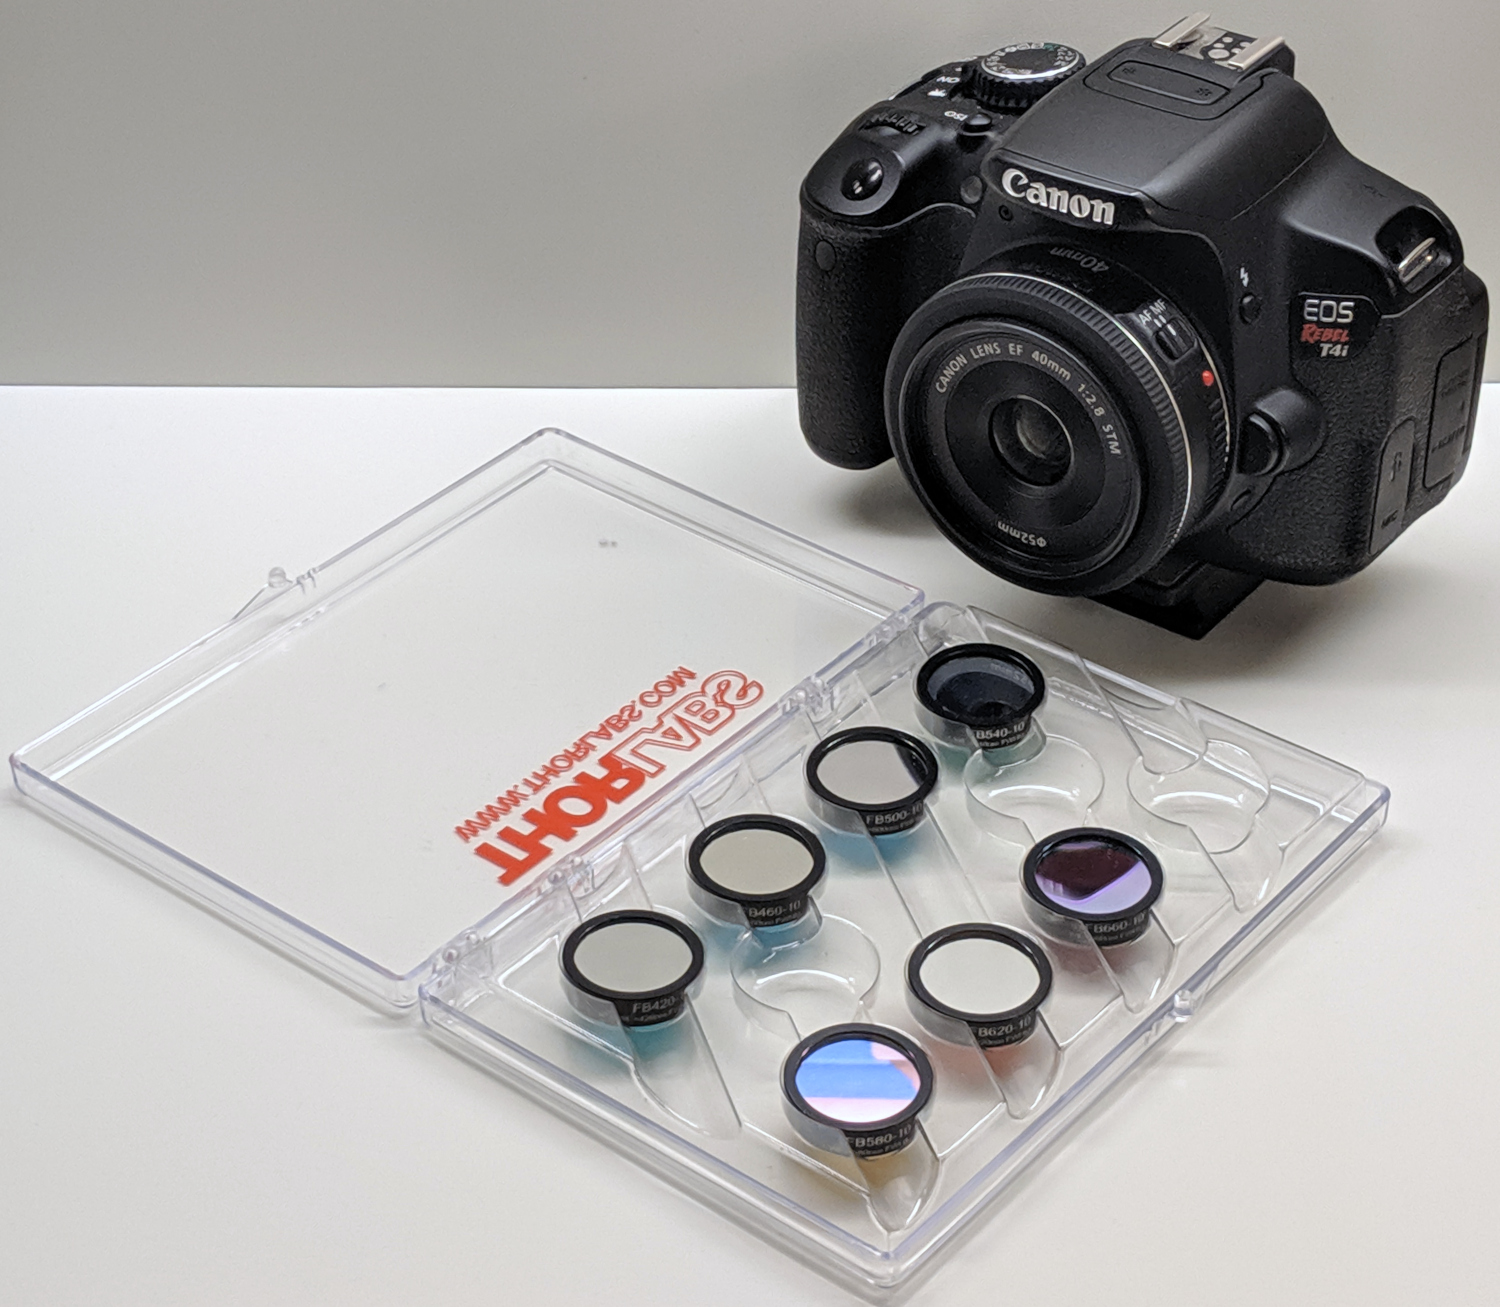
\includegraphics[width=0.45\textwidth]{IMG_20210712_212507_GIMP.jpg}
\caption{Placeholder text}
\label{canon}
\end{figure}

The open-source \texttt{dcraw} utility is used to extract RAW values stored in the .CR2 file format. The modifier string \texttt{-D -4 -j -t 0} specifies that the extracted RAW values are unprocessed sensor measurements:\\

\begin{tabular}{l | l}
-D & No value scaling \\
-4 & Linear 16-bit \\
-j & No stretching or rotating pixels \\
-t 0 & No image rotation \\
\end{tabular} \\

 The RAW sensor measurements are then demosaiced into R, G, B color channels with a Bayer filter pattern of \texttt{rggb}.

\subsection{SPD Measurements from RAW Photo Values}

 By rearranging the general expression of sensitivity in Section \ref{Camera_Spectral_Sensitivity}: \\

 $V_A = \dfrac{V_M}{S}$ \\

Assuming a linear sensor response, $V_M \propto P$, with $P$ denoting the RAW photo value. By inspection, $V_A \propto SPD$. Filter transmission $T$ is accounted for as a factor acting on $S$, a property of the camera only. Using proportionality and non-dimensionality, this is rearranged and substituted as: \\

 $SPD = V_A = \dfrac{P}{ST}$ \\

Accounting for the non-zero bandwidth of the filters, the denominator $ST$ is most accurately and generally expressed as $S(\lambda) \cdot T(\lambda)$, rather than $S(\lambda=CWL)*T(\lambda=CWL)$.

\id At an arbitrary pixel and CWL, each color channel produces an independent SPD measurement, collectively given as: \\

 $SPD = \left[ \dfrac{P_R}{S_R \cdot T},\dfrac{P_G}{S_G \cdot T},\dfrac{P_B}{S_B \cdot T} \right] $ \\

These measurements are theoretically equal, but in practice differ as a result of various sources of error. They are fused as a sensitivity-weighted average: \\

$\overline{SPD} = \dfrac{1}{S_R+S_G+S_B} \left( \dfrac{P_R S_R}{S_R \cdot T} + \dfrac{P_G S_G}{S_G \cdot T} + \dfrac{P_B S_B}{S_B \cdot T} \right)$\\

%with $\odot$ denoting element-wise product and $\cdot$ denoting dot product. This simplifies to:\\

% $\overline{SPD} = \dfrac{P_R+P_G+P_B}{T(S_R+S_G+S_B)} =  \dfrac{\mathlarger{\sum_{R,G,B}}P}{T \mathlarger{\sum_{R,G,B}}S}$ \\

Calculating $\overline{SPD}$ as a sensitivity-weighted average continuously interpolates between color channels as a function of wavelength, without discontinuities or switching behavior. Since $S_R+S_G+S_B > 0$ for all $\lambda$, divide-by-zero is precluded. This formulation generalizes efficiently from a 0D pixel to a 2D channel simply by using matrices in place of scalars for $P$.

\id The HSDC is first calculated in a sparse fashion, only at the CWLs of the filters. The full (i.e. non-sparse) HSDC is then calculated by means of 3D cubic interpolation in the wavelength domain between the filter CWLs, as discussed in Section \ref{curve_reconstruction}.

\subsection{Validation}

The system is validated by comparing measured SPDs from camera vs. spectrophotometer, taken as ground truth. The latter is modeled as $I(\lambda)R(\lambda)$, the element-wise product of the scene illuminant, taken as CIE D65, with the reflectance of the swatch. Results are shown in Figure \ref{SPD_validation}, showing good agreement. Error occurs mostly at high brightness and near the limits of the visible light spectrum, where sensitivity is lowest.

\subsection{Images from HSDCs}

 RGB images can be generated from HSDCs using standard CIE observer functions that relate an SPD to an XYZ tristimulus, which may then be converted to an RGB color for display. In the latter step, an \emph{a priori} value scaling method is needed to translate the non-dimensional colors from $\overline{SPD}$ to a dimensional color space. A robust general-purpose method is to scale the image's value limits by specifying two CDF pairs; for example:\\

Value(CDF = 1\%) = 5\%\\
Value(CDF = 99\%) = 95\%\\

However, observer functions have inherent limitations as the sole basis for generating RGB images from HSDCs. This is because they model independent single-color perception only, and do not account for the the mutual influence of simultaneously-perceived colors. This deficiency can be seen in nontrivial scenes where the luminance spans more orders of magnitude than the color space, or the illuminant is significantly non-spectrally uniform, i.e. colored; examples include sunsets and indoor incandescent lighting. Literature is presently lacking in research and methods for generating perceptually realistic images from nontrivial HSDCs.

\section{Discussion}

Placeholder text here

\clearpage

\onecolumn

\section{Results}

\begin{figure}[H]
\begin{centering}
  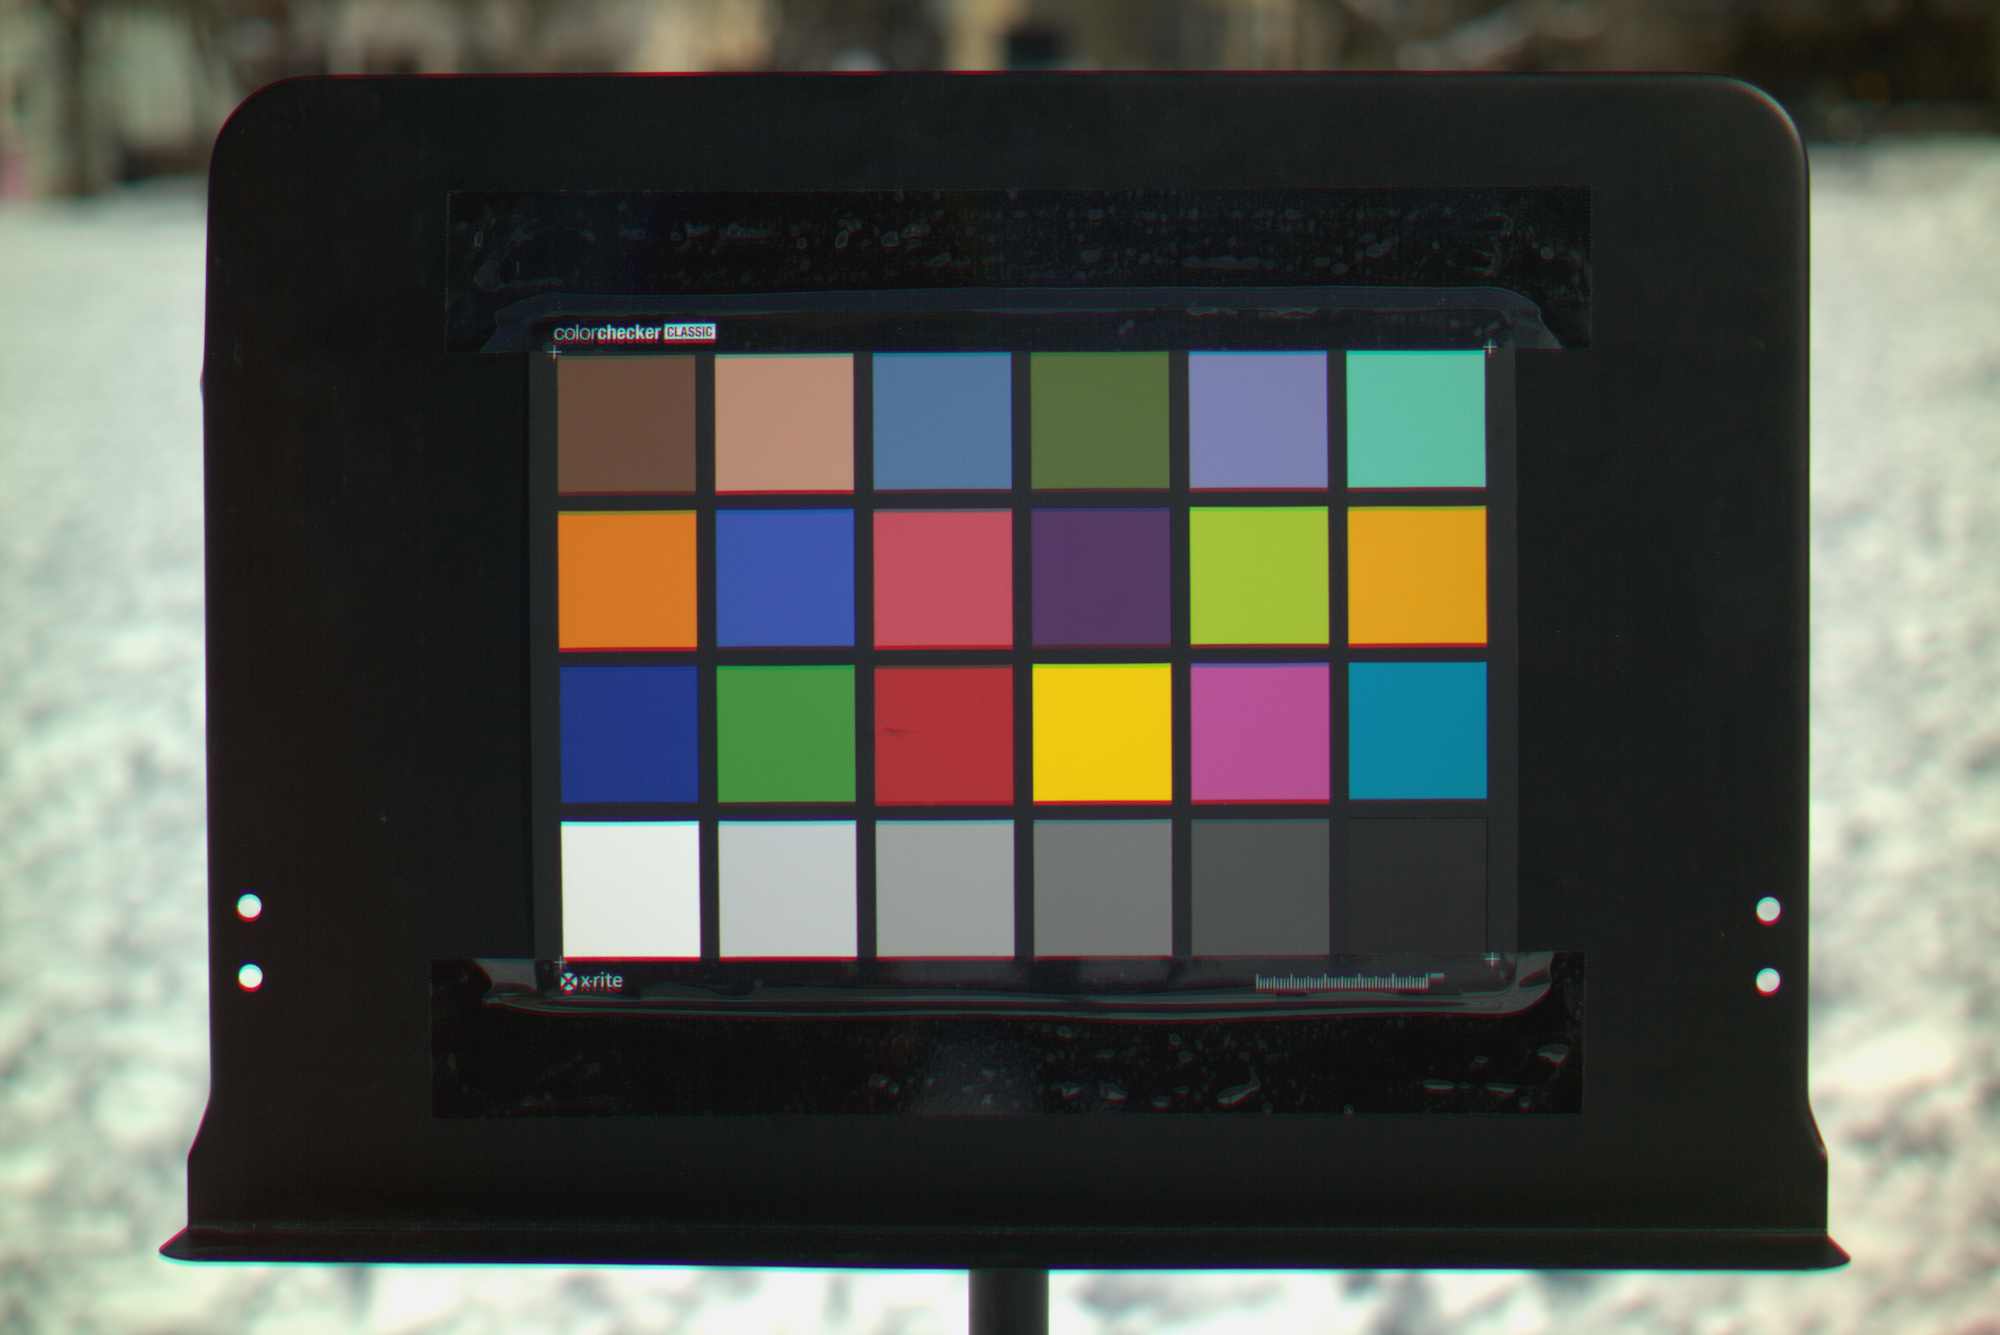
\includegraphics[height=0.55\linewidth]{colorchecker.png}
  \caption{Reconstructed image of ColorChecker chart under noon daylight. Mesh sample points overlaid as black-and-white circles.}
  \label{colorchecker_mesh}
  \end{centering}
\end{figure}

\begin{figure}[H]
\begin{centering}
  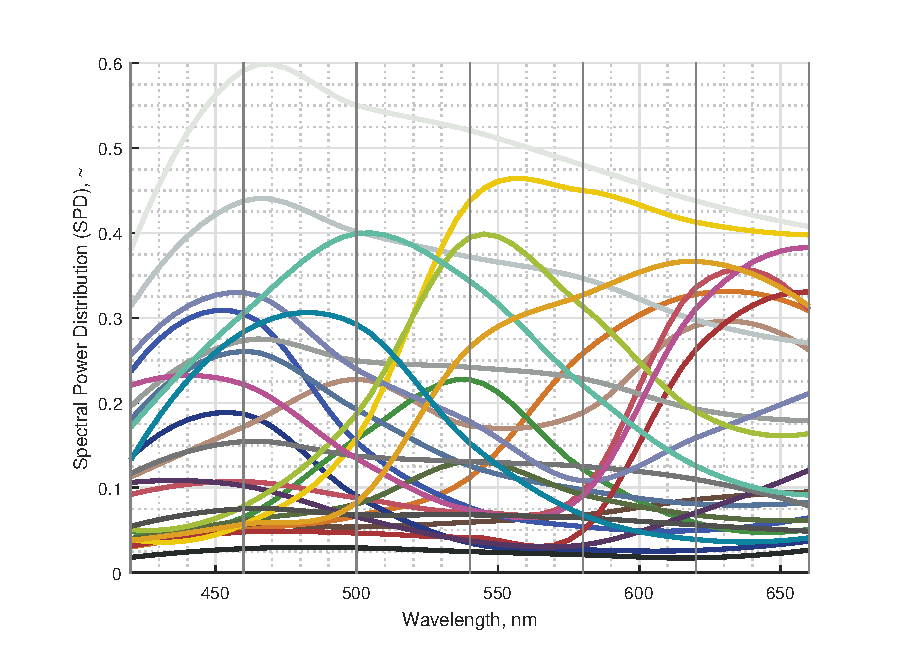
\includegraphics[height=0.6\linewidth]{colorchecker.eps}
  \caption{SPD curves at mesh points in Figure \ref{colorchecker_mesh}.}
  \label{colorchecker_SPDs}
    \end{centering}
\end{figure}

\clearpage


\begin{figure}[H]
\begin{centering}
  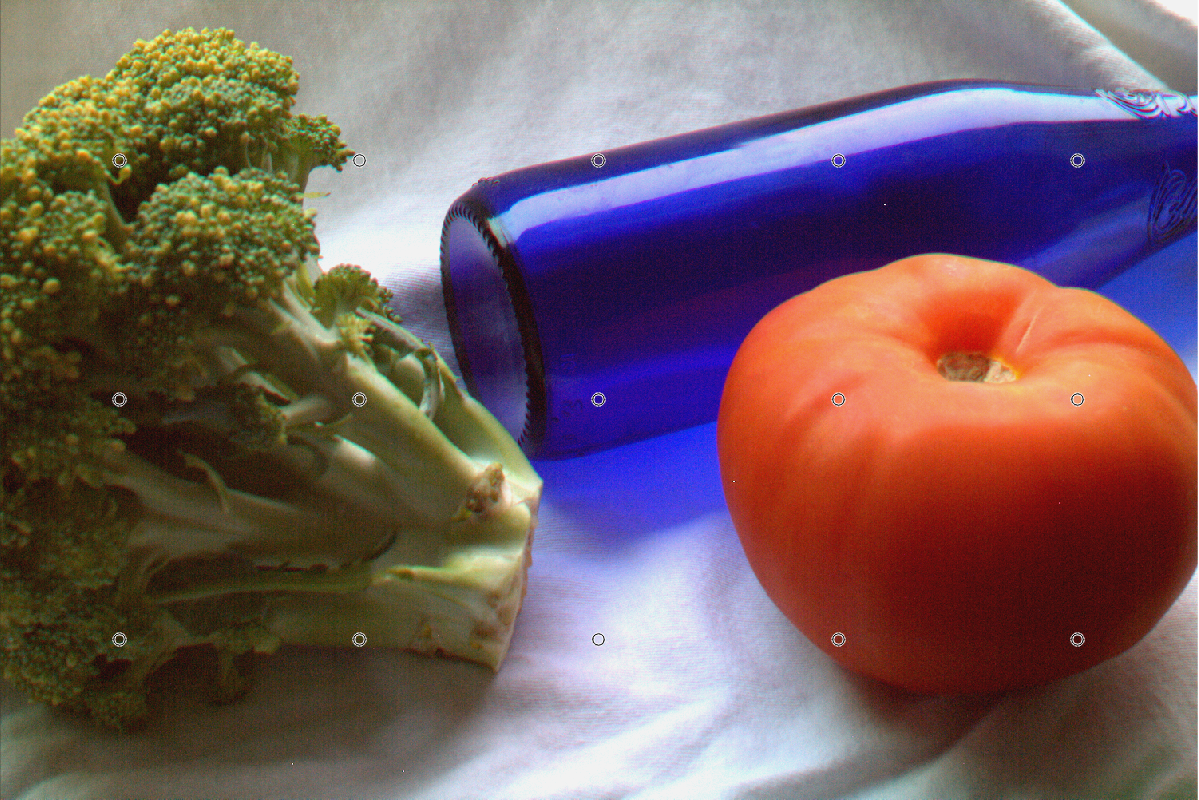
\includegraphics[height=0.55\linewidth]{broccoli_bottle_tomato.png}
  \caption{Placeholder text here}
  \label{tomato_mesh}
  \end{centering}
\end{figure}

\begin{figure}[H]
\begin{centering}
  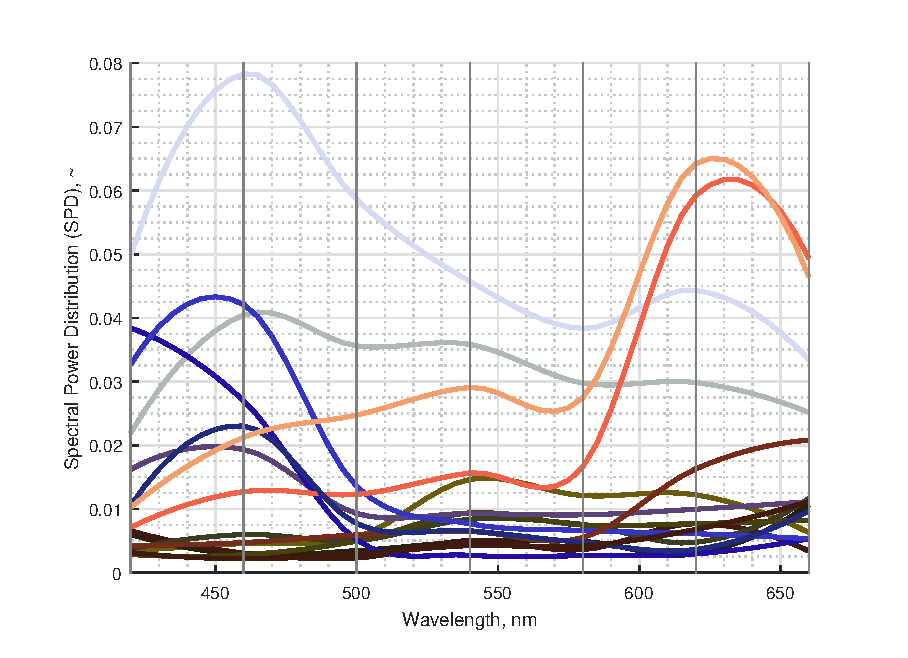
\includegraphics[height=0.6\linewidth]{broccoli_bottle_tomato.eps}
  \caption{Placeholder text here}
  \label{tomato_SPDs}
  \end{centering}
\end{figure}

\clearpage

\begin{figure}[H]
\begin{centering}
  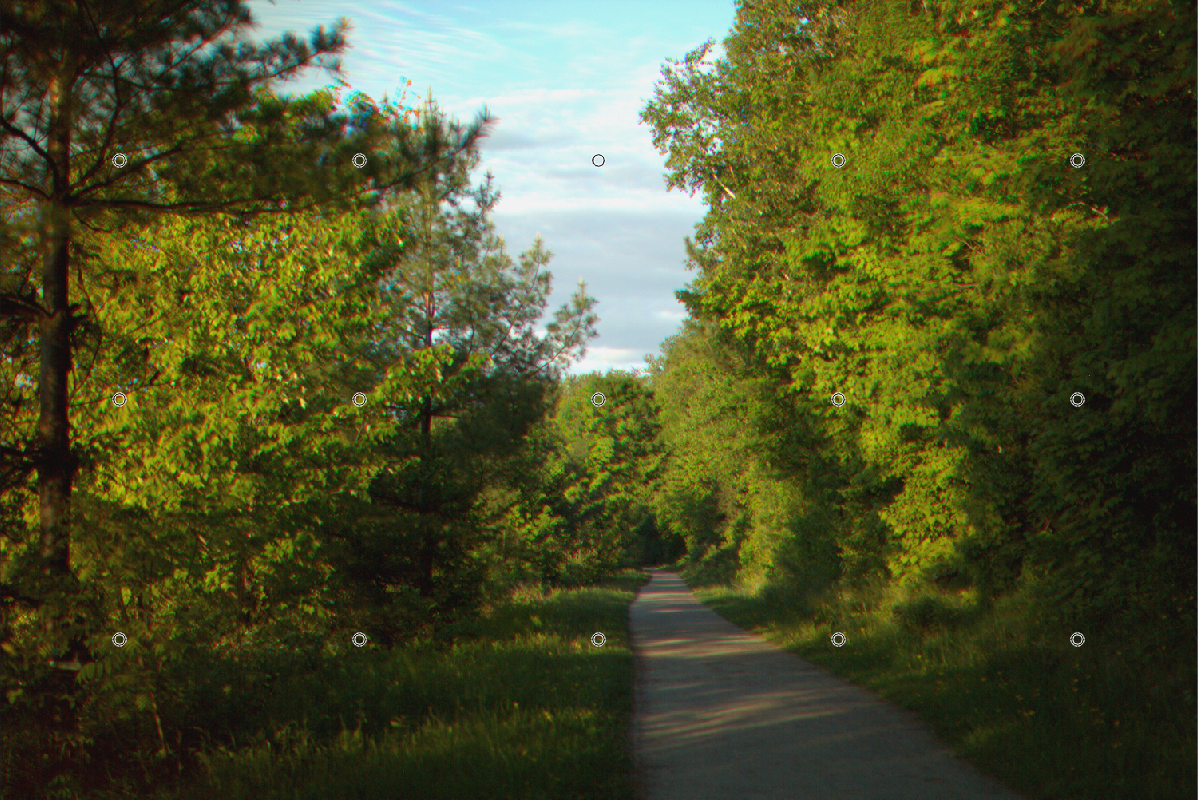
\includegraphics[height=0.55\linewidth]{vermont_path.png}
  \caption{Placeholder text here}
  \label{tomato_mesh}
  \end{centering}
\end{figure}

\begin{figure}[H]
\begin{centering}
  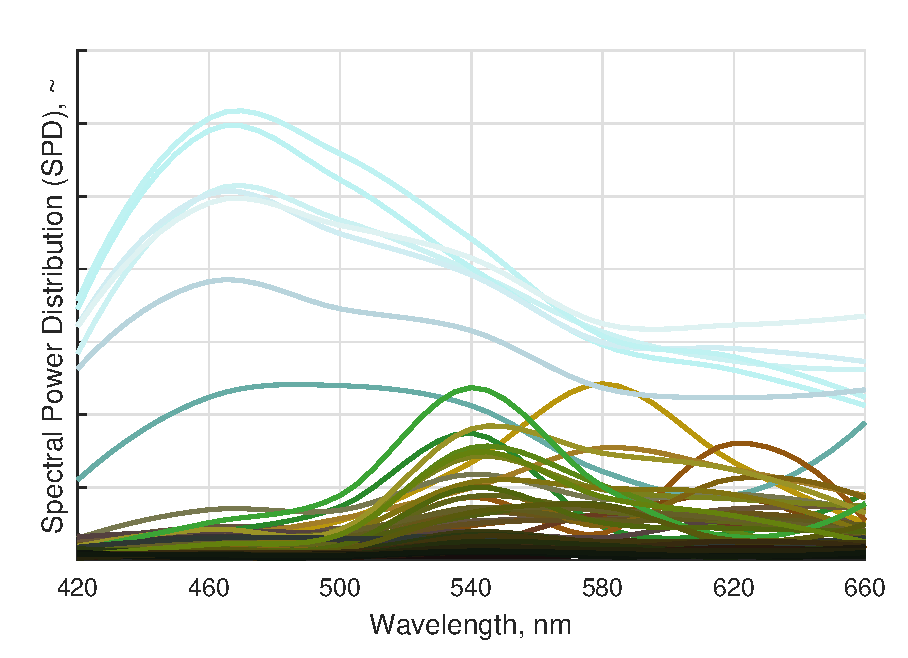
\includegraphics[height=0.6\linewidth]{vermont_path.eps}
  \caption{Placeholder text here}
  \label{tomato_SPDs}
  \end{centering}
\end{figure}

\clearpage

\section{Appendix}
\label{appendix}

\begin{figure}[H]
\begin{centering}
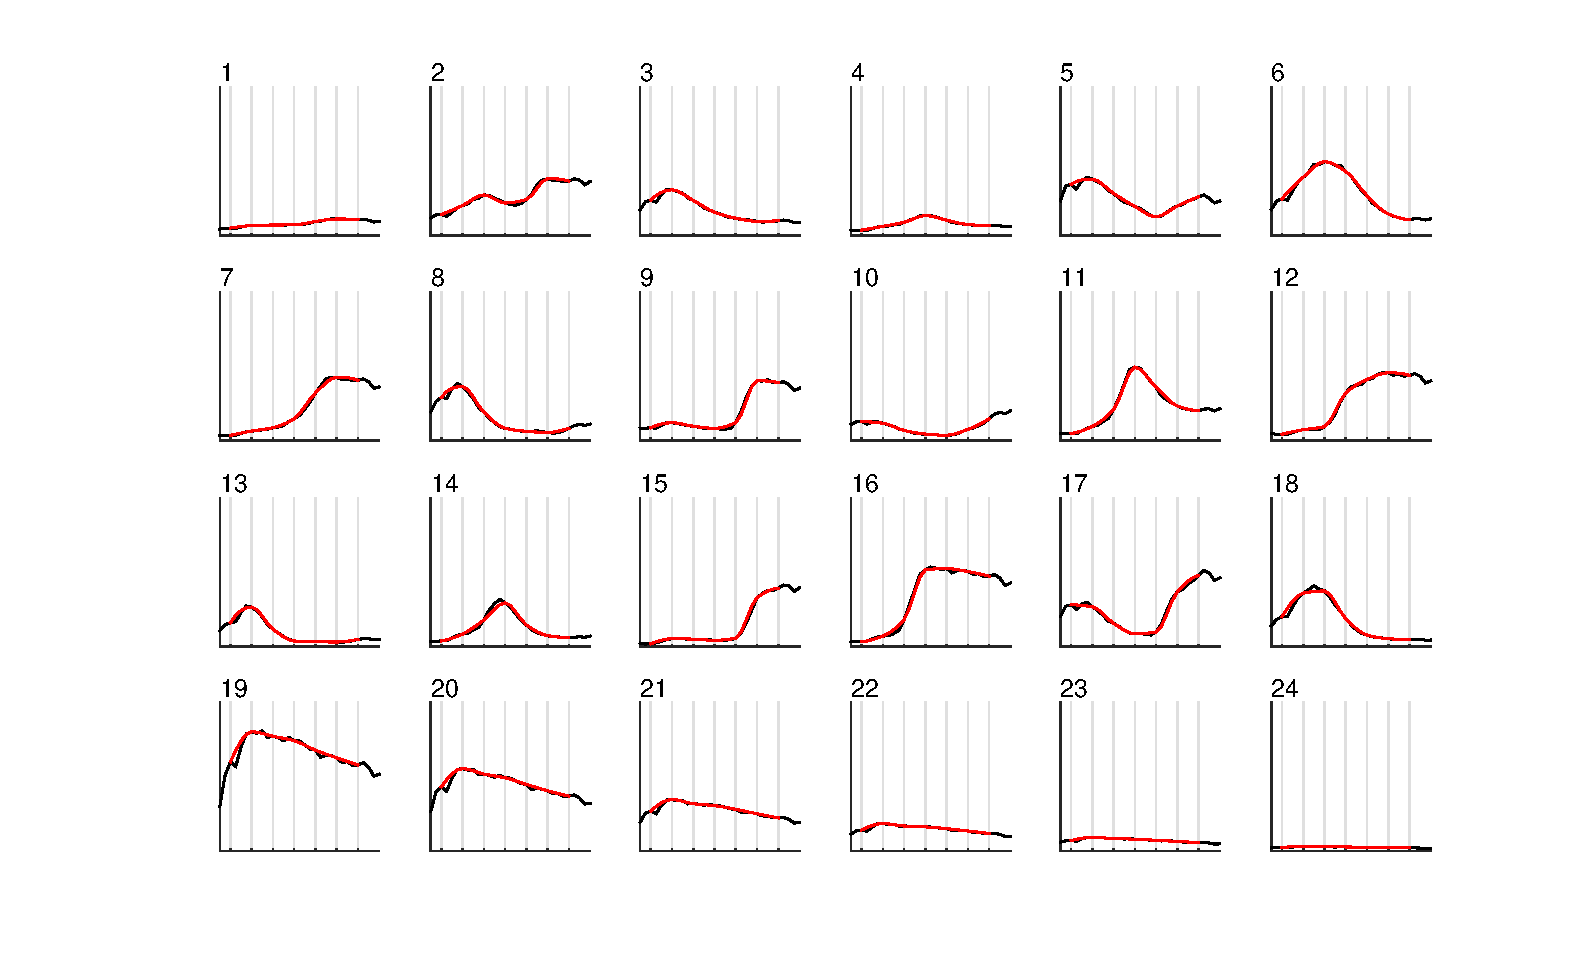
\includegraphics[width=0.90\textwidth]{colorchecker_reconstruction.eps}
\caption{Curve reconstruction of simulated SPDs from ColorChecker measured reflectance spectra under D65 illuminant, with cubic interpolation, and 7 samples at 40 nm starting at 420 nm. All plots are scaled BLANK to BLANK.}
\label{colorchecker_reconstruction}
\end{centering}
\end{figure}



\begin{figure}[H]
\centering
  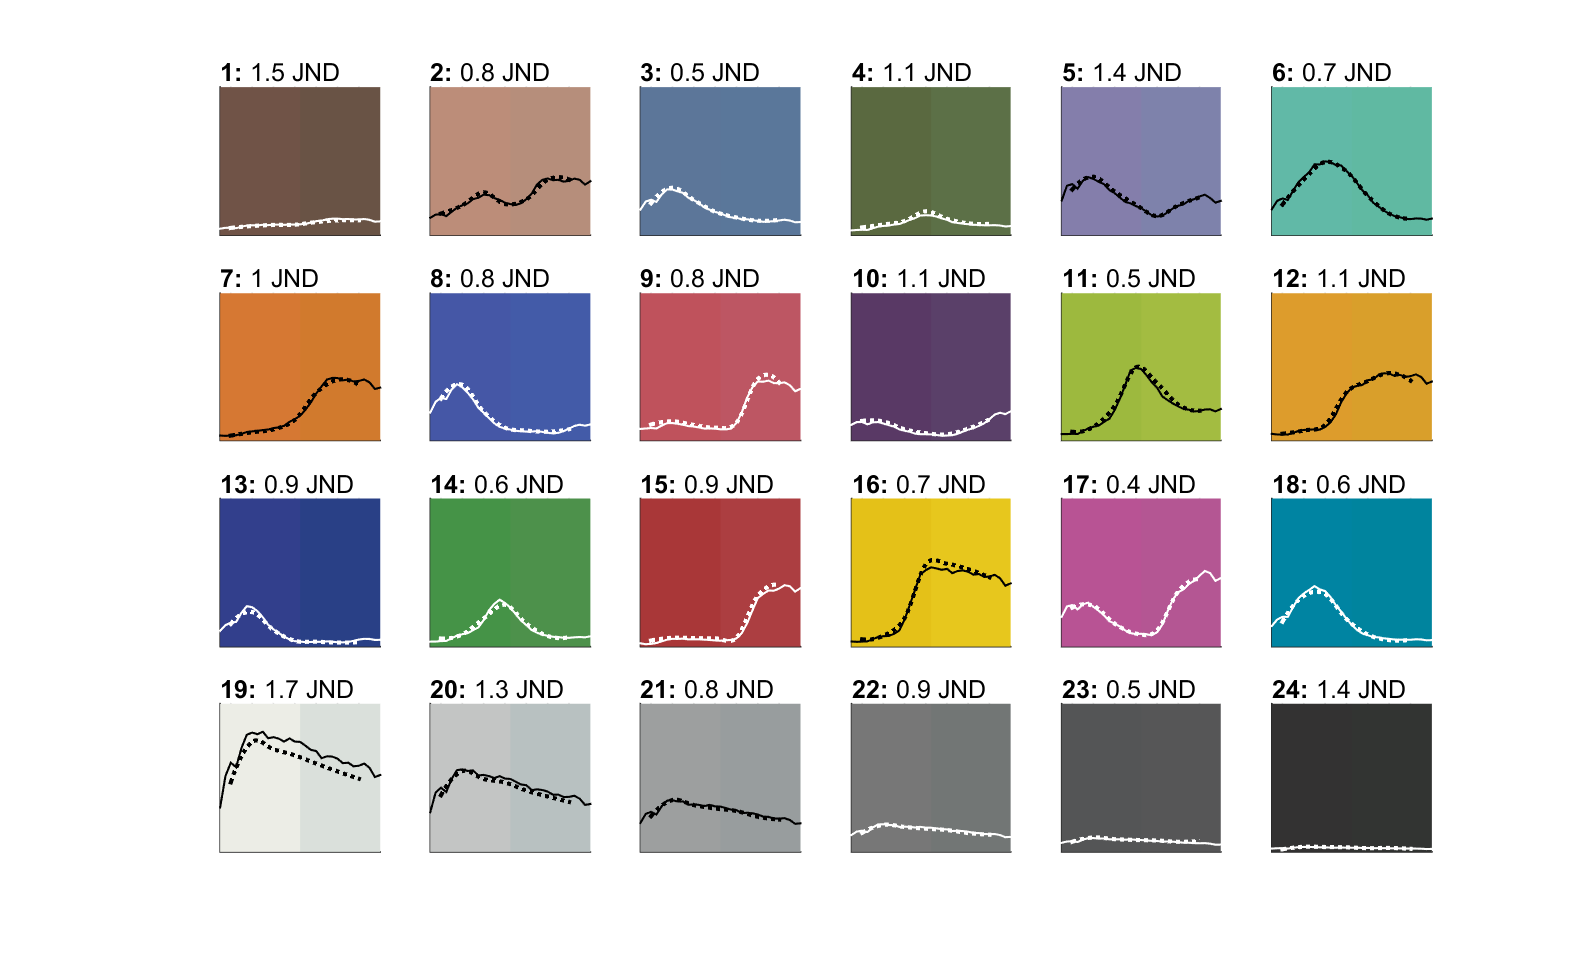
\includegraphics[width=0.90\linewidth]{SPD_validation.eps}
  \caption{Comparison of SPDs from camera (red) and from direct measurement (black) for the ColorChecker dataset. Filter CWLs are shown as gray vertical lines. Plots are scaled 400 to 700 nm along x, and non-dimensional along y. A single scalar gain is applied to align the magnitudes of the two sets of curves.}
  \label{SPD_validation}
\end{figure}




\begin{table}[t]
\begin{center}
\begin{tabular}{l l r l r}
\hline
\textbf{Reflectance Dataset} & \textbf{Illuminant} & \textbf{Resolution, nm} & \textbf{Interpolation Method} & \textbf{Error Metric} \\
\hline
Parkkinen & None & 30 & spline & 0.024  \\
Parkkinen & None & 30 & cubic  & 0.038  \\
Parkkinen & None & 30 & linear & 0.053  \\
Parkkinen & None & 40 & cubic  & 0.068  \\
Parkkinen & None & 40 & spline & 0.069  \\
Parkkinen & None & 40 & linear & 0.118  \\
\hline
ColorChecker & None & 30 & cubic  & 0.006  \\
ColorChecker & None & 30 & spline & 0.010  \\
ColorChecker & None & 40 & cubic  & 0.016  \\
ColorChecker & None & 30 & linear & 0.018  \\
ColorChecker & None & 40 & linear & 0.032  \\
ColorChecker & None & 40 & spline & 0.035  \\
\hline
Parkkinen & D65 & 30 & spline & 0.028  \\
Parkkinen & D65 & 30 & cubic  & 0.033  \\
Parkkinen & D65 & 30 & linear & 0.040  \\
Parkkinen & D65 & 40 & cubic  & 0.057  \\
Parkkinen & D65 & 40 & spline & 0.062  \\
Parkkinen & D65 & 40 & linear & 0.090  \\
\hline
ColorChecker & D65 & 30 & linear & 0.033  \\
ColorChecker & D65 & 40 & cubic  & 0.034  \\
ColorChecker & D65 & 30 & cubic  & 0.034  \\
ColorChecker & D65 & 30 & spline & 0.036  \\
ColorChecker & D65 & 40 & linear & 0.039  \\
ColorChecker & D65 & 40 & spline & 0.055  \\
\hline
\end{tabular}
\caption{Figure and table captions do not end with a period}
\label{table_reconstruction}
\end{center}
\end{table}

\clearpage

 \begin{thebibliography}{12}

 \bibitem{Parkkinen} 
 {Parkkinen, J. \& Hallikainen, J. \& Jääskeläinen, Timo. (1989). Characteristic spectra of Munsell chips. Journal of The Optical Society of America A-optics Image Science and Vision - J OPT SOC AM A-OPT IMAGE SCI. 6. 10.1364/JOSAA.6.000318.}
 
\bibitem{Jiang}
{J. Jiang, D. Liu, J. Gu and S. Süsstrunk, "What is the space of spectral sensitivity functions for digital color cameras?," 2013 IEEE Workshop on Applications of Computer Vision (WACV), 2013, pp. 168-179, doi: 10.1109/WACV.2013.6475015.}

\bibitem{Cosentino}
{Cosentino, Antonino. (2015). Multispectral Imaging of Pigments with a digital camera and 12 interferential filters. e-Preservation Science. 12. 1-7.}

\bibitem{Oh}
{S. W. Oh, M. S. Brown, M. Pollefeys and S. J. Kim, "Do It Yourself Hyperspectral Imaging with Everyday Digital Cameras," 2016 IEEE Conference on Computer Vision and Pattern Recognition (CVPR), 2016, pp. 2461-2469, doi: 10.1109/CVPR.2016.270.}

\bibitem{Baek}
{Seung-Hwan Baek, Incheol Kim, Diego Gutierrez, and Min H. Kim. 2017. Compact single-shot hyperspectral imaging using a prism. ACM Trans. Graph. 36, 6, Article 217 (November 2017), 12 pages. DOI: https://doi.org/10.1145/3130800.3130896}

\bibitem{Habel}
{Habel, R. et al. “Practical Spectral Photography.” Computer Graphics Forum 31 (2012): n. pag.}

 \end{thebibliography}
 
 

\end{document}
